\documentclass[aspectratio=169,10pt]{beamer}

\usetheme{Madrid}
\usecolortheme{seahorse}
\useinnertheme{rectangles}
\setbeamertemplate{navigation symbols}{}
\setbeamertemplate{caption}[numbered]

\usepackage[utf8]{inputenc}
\usepackage[T1]{fontenc}
\usepackage[english]{babel}
\usepackage{amsmath,amssymb,amsthm}
\usepackage{booktabs}
\usepackage{array}
\usepackage{multirow}
\usepackage{tikz}
\usetikzlibrary{positioning,arrows.meta,shapes,fit,backgrounds}
\usepackage{hyperref}
\usepackage{graphicx}
\usepackage{siunitx}

% Custom colors
\definecolor{darkblue}{RGB}{0,51,102}
\definecolor{darkred}{RGB}{153,0,0}
\definecolor{darkgreen}{RGB}{0,102,51}

% Shortcuts
\newcommand{\onecite}[1]{\textcolor{darkblue}{\textsc{#1}}}
\newcommand{\hl}[1]{\textcolor{darkred}{\textbf{#1}}}

\title[Lei 13.811/2019]{Evaluating the 2019 Child Marriage Ban in Brazil}
\subtitle{Mechanisms, a Marriage Market Model, and Identification Strategy}
\author[Research Team]{Research Team}
\institute{Research Design Note for Coauthor Discussion}
\date{April 2026}

\begin{document}

% =============================================================
\begin{frame}
    \titlepage
\end{frame}

% =============================================================
% OPENING SEQUENCE: law regimes + expected CDFs
% Narrative arc: observation -> baseline -> reform -> H1 -> H2
% Figures live in ../output/; rename path to figures/ if needed.
% =============================================================

% ------ Frame 1: legal regime before 2019 --------------------
\begin{frame}{Motivation}
    \begin{block}{Before Lei 13.811/2019: a permissive regime below age 16}
        \small
        Art.~1.520 of the Civil Code allowed a judge to grant marriage
        \textit{below age 16} in two circumstances: (i)~pregnancy, or
        (ii)~to avoid criminal prosecution of the groom.
        No minimum age floor existed --- exceptions were granted case by case.
    \end{block}
    \vspace{0.15cm}
    \begin{center}
        
\includegraphics[width=\linewidth]{../output/plot1_law_pre2019.pdf}
    \end{center}
\end{frame}

% ------ Frame 2: expected formal CDF pre-2019 ----------------
\begin{frame}{Motivation}
    \begin{block}{Baseline distribution of formal marriages before 2019}
        \small
        Under this regime, \textasciitilde{}85\% of formal child marriages
        are concentrated at ages 16--17 (parental-consent zone), but the
        exception clause generates a \hl{small tail below age 16}.
        This tail is our pre-reform baseline --- it should vanish after 2019
        \textit{if} the ban is enforced.
    \end{block}
    \vspace{0.15cm}
    \begin{center}
        
\includegraphics[width=\linewidth]{../output/plot2_cdf_formal_pre2019.pdf}
    \end{center}
\end{frame}

% ------ Frame 3: legal regime after 2019 ---------------------
\begin{frame}{Motivation}
    \begin{block}{Lei 13.811/2019: an unconditional prohibition below age 16}
        \small
        Enacted 12 March 2019, the law eliminated \textit{all} exceptions ---
        formal marriage below age 16 is now \hl{absolutely prohibited} under
        any circumstance.
        This creates a \textbf{clean, well-defined treatment threshold}:
        a hard age floor with no judicial discretion.
    \end{block}
    \vspace{0.15cm}
    \begin{center}
        
\includegraphics[width=\linewidth]{../output/plot3_law_post2019.pdf}
    \end{center}
\end{frame}

% ------ Frame 4: H1 -- formal marriages -----------------------
\begin{frame}{Motivation}
    \begin{alertblock}{Hypothesis 1 --- Formal marriages below 16 should drop to zero}
        \small
        Under full enforcement, the Registro Civil should show \textbf{no}
        formal marriages below age 16 after 2019.
        We test this with an event study on the formal-marriage hazard
        and a McCrary bunching test at the legal threshold.
        Any residual mass below 16 in administrative data signals
        \hl{non-compliance or evasion}.
    \end{alertblock}
    \vspace{0.15cm}
    \begin{center}
        
\includegraphics[width=\linewidth]{../output/plot4_cdf_formal_post2019.pdf}
    \end{center}
\end{frame}

% ------ Frame 5: H2 -- informal unions -----------------------
\begin{frame}{Motivation}
    \begin{alertblock}{Hypothesis 2 --- Informal unions are outside the law's reach}
        \small
        The civil-registry ban covers \textit{only} formal marriages.
        Informal unions --- \hl{89.5\% of child unions} (Census 2010) ---
        are legally unreachable.
        If families substitute from formal to informal channels, the
        informal CDF should be \textbf{unchanged or larger} after 2019.
        Divergence between the two margins identifies
        \textbf{real reduction} vs.\ \textbf{displacement}.
    \end{alertblock}
    \vspace{0.15cm}
    \begin{center}
        
\includegraphics[width=\linewidth]{../output/plot5_cdf_informal_comparison.pdf}
    \end{center}
\end{frame}

% =============================================================
\begin{frame}{Outline}
    \tableofcontents
\end{frame}

% =============================================================
\section{Motivation and Research Question}

\begin{frame}{Motivation}
    \begin{itemize}
        \item Brazil ranks \hl{fourth worldwide} in absolute number of women married as children (Margarido 2024).
        \item \hl{Lei 13.811/2019} eliminated all exceptions to the minimum marriage age of 16 --- previously, pregnancy or avoidance of criminal prosecution permitted marriage below 16.
        \item Yet formal and informal child unions persist: Registro Civil 2021 records \hl{45.4 girls married per day} formally (Margarido 2024).
        \item Global evidence on minimum-age laws is mixed: some bind (Bharadwaj 2015), many fail to enforce (Collin 2016); administrative data systematically overstates law effects (Blank 2020).
    \end{itemize}
    \vspace{0.3cm}
    \centering
    \textit{Did the 2019 ban actually reduce child marriage in Brazil --- and which marriages persisted?}
\end{frame}

% =============================================================
\begin{frame}{Research Questions}
    \begin{block}{Primary question}
        Did Lei 13.811/2019 causally reduce child marriage in Brazil, and through which margins (formal vs. informal, age, region)?
    \end{block}

    \begin{block}{Secondary questions}
        \begin{enumerate}
            \item What \hl{mechanisms} sustain child marriage in Brazil --- economic pressure, normative pressure, or both?
            \item Which marriages are \hl{elastic to income policy} (e.g., Bolsa Fam\'ilia) vs. \hl{inelastic} (norm-driven, enforcement-proof)?
            \item Can we quantify a \hl{``norm-irreducible'' share} of child marriages that legal and economic interventions alone cannot reach?
        \end{enumerate}
    \end{block}

    \begin{block}{Contribution}
        First causal evaluation of Lei 13.811/2019 combining a marriage-market model, heterogeneous-mechanism estimation, and formal/informal margin comparison.
    \end{block}
\end{frame}

% =============================================================
\begin{frame}{Legal Context: Lei 13.811/2019}
    \begin{columns}[T]
        \column{0.5\textwidth}
        \textbf{Before 12 March 2019} (Art.~1.520, CC):
        \begin{itemize}
            \item Minimum marriage age: 16 with parental consent; 18 without.
            \item \hl{Exceptions below 16}: pregnancy or to avoid criminal prosecution of the groom.
        \end{itemize}

        \column{0.5\textwidth}
        \textbf{After Lei 13.811/2019}:
        \begin{itemize}
            \item Absolute minimum: 16 (with parental consent).
            \item \hl{No exceptions}.
            \item Informal unions remain legally unregulated.
        \end{itemize}
    \end{columns}

    \vspace{0.4cm}
    \begin{alertblock}{Key enforcement concern}
        The law only affects \textit{formal} marriages. Informal unions, which constitute \hl{89.5\% of child unions} in the 2010 Census (Margarido 2024), fall outside civil registry jurisdiction.
    \end{alertblock}
\end{frame}

% =============================================================
\section{Child Marriage in Brazil: Stylized Facts}

\begin{frame}{Stylized Facts (I): Prevalence and Demographics}
    \begin{itemize}
        \item \onecite{Cardoso et al.\ 2022} (PNS 2013): \hl{3.9\% prevalence} of union before 18 among under-18s; overwhelmingly female, Black/brown, lower-income, Northern/Northeastern.
        \item \onecite{Margarido 2024} (Census 2010): \hl{655{,}935 children} in some form of union; girls outnumber boys 5:1; \hl{89.5\% informal}.
        \item \onecite{Pinto et al.\ 2024} (SINASC 2011--2021): \hl{127{,}022 live births} to mothers aged 10--14; \hl{21.1\%} declared married or in stable union. Moran's I = 0.47 --- strong spatial clustering in North and Center-West.
        \item \onecite{Aguiar et al.\ 2025} (SINAN 2014--2021): \hl{3{,}681 cases} of marital rape of girls $\leq$14; 61\% recurrent; concentrated in Acre, Pernambuco, Par\'a, Amazonas.
    \end{itemize}
\end{frame}

% =============================================================
\begin{frame}{Stylized Facts (II): Who, Where, Why}
    \begin{columns}[T]
        \column{0.5\textwidth}
        \textbf{Who}
        \begin{itemize}
            \item Girls, ages 12--17 (mode 14--15)
            \item Black/brown (65--75\% across studies)
            \item Lower household education and income
            \item Often pregnant at time of union formation
        \end{itemize}

        \textbf{Where}
        \begin{itemize}
            \item Rural North and Northeast
            \item Center-West emerging (Pinto 2024)
            \item Peripheries of major cities (Margarido 2021)
        \end{itemize}

        \column{0.5\textwidth}
        \textbf{Why (qualitative evidence)}
        \begin{itemize}
            \item Control of female sexuality / family honor \\ (Taylor \& Fonseca 2015)
            \item Poverty / ``exit option'' \\ (Veiga \& Zanello 2020)
            \item Pregnancy ``repair'' union \\ (Taylor \& Fonseca 2015)
            \item Normalization via social media \\ (Huhn 2022)
            \item Intergenerational transmission \\ (Asadullah 2018, globally)
        \end{itemize}
    \end{columns}
\end{frame}

% =============================================================
\begin{frame}{Stylized Facts (III): What the PBF Evidence Already Tells Us}
    \onecite{Vasconcelos \& Griebeler (2017, 2023)} use Propensity Score Matching on PNADC data:
    \begin{itemize}
        \item Bolsa Fam\'ilia \hl{reduces child marriage} among poor and extremely poor girls.
        \item \hl{Protective effect is concentrated at ages 16--18}.
        \item \hl{Null effect at 14--15}: income transfers do not move the youngest unions.
    \end{itemize}
    \vspace{0.3cm}
    \begin{alertblock}{Interpretation}
        The age-heterogeneity in PBF response is already \hl{prima facie evidence} that a large share of the youngest marriages are driven by mechanisms other than economic pressure --- the same mechanisms a legal ban would need to reach.
    \end{alertblock}
\end{frame}

% =============================================================
\section{Literature: Global vs.\ Brazilian}

\begin{frame}{Global Literature --- Core Findings}
    \small
    \begin{tabular}{p{3.2cm} p{3cm} p{7cm}}
        \toprule
        \textbf{Study} & \textbf{Context / Method} & \textbf{Key finding} \\
        \midrule
        Field \& Ambrus (2008) & Bangladesh / menarche IV & +1 yr marriage delay $\rightarrow$ +0.22 yr schooling \\
        Dahl (2010) & USA / state law IV & Early marriage $\rightarrow$ +31 pp poverty for women \\
        Bharadwaj (2015) & Mississippi 1957 / DiD & Law reform: $-75\%$ marriages, $+3\%$ enrollment \\
        Duflo et al.\ (2015) & Kenya / RCT & Education subsidy beats HIV education for delay \\
        Wahhaj (2015) & Bangladesh / OLG model & Reputational equilibrium sustains early marriage \\
        Ashraf et al.\ (2016) & Indonesia / Zambia & School supply binds in bride-price groups only \\
        Collin \& Talbot (2016) & 60+ countries & Most minimum-age laws poorly enforced \\
        Kidman (2016) & 34 countries / DHS & Child marriage $\rightarrow$ OR $\approx$ 1.5 for IPV \\
        Chari et al.\ (2017) & India / menarche IV & Intergenerational: +3.1\% child school enrollment \\
        Corno et al.\ (2019) & SSA vs.\ India & Bride price $\uparrow$ vs.\ dowry $\downarrow$ under droughts \\
        Blank et al.\ (2020) & USA / admin vs.\ survey & Admin data overstates law effects \\
        Chow \& Vivalt (2022) & Ethiopia / DiD & Community interventions reduce marriage 4--7 pp \\
        Wilson (2022) & LMICs / DiD & Age-18 bans raise marriage age, first-birth age, employment \\
        \bottomrule
    \end{tabular}
\end{frame}

% =============================================================
\begin{frame}{Brazilian Literature --- Core Findings}
    \small
    \begin{tabular}{p{3.2cm} p{3cm} p{7cm}}
        \toprule
        \textbf{Study} & \textbf{Data / Method} & \textbf{Key finding} \\
        \midrule
        Taylor \& Fonseca (2015) & Par\'a/Maranh\~ao / mixed & Honor, sexuality control, pregnancy trigger unions \\
        Vasconcelos \& Griebeler (2017) & PNADC / PSM & PBF protects girls in extreme poverty \\
        Veiga \& Zanello (2020) & Goi\'as / qualitative & ``Choosing and being chosen''; constrained agency \\
        Cargnin et al.\ (2021) & Rio Branco / SINAN & 41.2\% of 10--14 yr sexual-violence victims in union \\
        Margarido (2021) & S\~ao Paulo / ethnography & Protection-network failures in metropolitan periphery \\
        Cardoso et al.\ (2022) & PNS 2013 / Poisson & 3.9\% prevalence; intersectional determinants \\
        Huhn (2022) & Digital ethnography & Social media normalizes the practice \\
        Vasconcelos \& Griebeler (2023) & PNADC / PSM & PBF effect concentrated at 16--18; null at 14--15 \\
        Margarido (2024) & Census + Registro Civil & 655k unions (Census); 45.4 formal marriages/day (2021); agency typology \\
        Pinto et al.\ (2024) & SINASC / spatial & Moran's I = 0.47; North/Center-West clusters \\
        Aguiar et al.\ (2025) & SINAN / multivariate & 3{,}681 marital rapes of girls $\leq$14 (2014--2021) \\
        \bottomrule
    \end{tabular}
\end{frame}

% =============================================================
\begin{frame}{Contrasting the Two Literatures}
    \begin{tabular}{p{4cm} p{5cm} p{5cm}}
        \toprule
        \textbf{Dimension} & \textbf{Global literature} & \textbf{Brazilian literature} \\
        \midrule
        Causal identification & Strong (IV, DiD, RCT) & Mostly descriptive / PSM \\
        Economic mechanism & Bride price, dowry, income shocks & Poverty as exit option; PBF \\
        Norm mechanism & Formal equilibrium models (Wahhaj) & Qualitative, ethnographic \\
        Violence & IPV as outcome (Kidman) & Central frame (SINAN, SINASC) \\
        Race/class & Rarely foregrounded & Intersectionality central \\
        Agency & Girls as passive & Rich constrained-agency theory \\
        Law enforcement & Quantitatively skeptical & Institutionally skeptical \\
        \bottomrule
    \end{tabular}
    \vspace{0.3cm}
    \begin{block}{Our opportunity}
        Import global causal-identification tools into the richer Brazilian descriptive, health-system, and intersectional framing --- and close the methodological gap.
    \end{block}
\end{frame}

% =============================================================
\section{Mechanisms: A 2$\times$2 Typology}

\begin{frame}{Mechanisms: the 2$\times$2 Typology}
    \small
    \centering
    \renewcommand{\arraystretch}{1.6}
    \begin{tabular}{l|p{4.5cm}|p{4.5cm}}
         & \textbf{Low normative pressure} & \textbf{High normative pressure} \\
        \hline
        \textbf{High economic pressure} & \textbf{Type A: Pure poverty} \newline Income policy eliminates marriage. PBF bites. & \textbf{Type B: Reinforced} \newline Income policy partially reduces. \\
        \hline
        \textbf{Low economic pressure} & \textbf{Type D: Neither} \newline Marriage unlikely. & \textbf{Type C: Pure norm} \newline Income policy has zero effect. Law may or may not bind. \\
    \end{tabular}

    \vspace{0.4cm}
    \begin{itemize}
        \item Vasconcelos \& Griebeler's \hl{null effect at ages 14--15} is consistent with a large share of Type C in that age window.
        \item A legal ban should, in principle, reach Types B and C --- \hl{if enforced}.
        \item Types B and C are also where post-pregnancy ``repair'' unions concentrate.
    \end{itemize}
\end{frame}

% =============================================================
\begin{frame}{Which Marriages Persist Under an Income Policy?}
    Expected to persist under a pure income policy (PBF or universal transfer):
    \begin{enumerate}
        \item \hl{Very young unions ($<$ 15)}: age floor itself is normative; income elasticity $\approx$ 0.
        \item \hl{Post-pregnancy ``repair'' unions}: causality runs pregnancy $\rightarrow$ marriage; transfers don't intervene in time.
        \item \hl{High-norm regions / families}: Northern interior, intergenerational transmission.
        \item \hl{Partner-coerced unions}: SINAN data (Aguiar 2025) shows perpetrator is often older, recurrent --- income to parents may be inert or counterproductive.
        \item \hl{Informal unions below legal threshold}: evade both Registro Civil and formal policy targeting.
    \end{enumerate}

    \vspace{0.2cm}
    \begin{block}{Testable implication for Lei 13.811/2019}
        If the 2019 ban reduces only formal marriages but leaves informal unions unchanged, it shifts margins without reducing total child marriage. This is the \hl{Collin (2016) / Blank (2020) concern} applied to Brazil.
    \end{block}
\end{frame}

% =============================================================
\section{A Model of the Brazilian Marriage Market}

\begin{frame}{Modeling Choices for the Brazilian Context}
    \begin{itemize}
        \item \hl{No formal bride price or dowry} --- rules out Corno (2019) sign-switching directly. Economic channel operates through consumption and labor.
        \item \hl{Pregnancy is a major trigger} of union formation (Taylor \& Fonseca 2015) --- must enter the model as a state variable.
        \item \hl{Informal $\gg$ formal} --- agents face a margin choice (formal vs.\ informal union), modulated by law.
        \item \hl{Agency is constrained but real} (Margarido 2024, Veiga \& Zanello 2020) --- decision is joint family--girl, not pure parental.
        \item \hl{Norms vary intergenerationally} --- usable as identification variation.
    \end{itemize}
\end{frame}

% =============================================================
\begin{frame}{A Discrete-Choice Marriage Timing Model}
    Household $i$ with daughter age $a \in \{10, 11, \dots, 17\}$. In each period decides: \emph{marry formally} ($M=F$), \emph{marry informally} ($M=I$), or \emph{wait} ($M=W$).
    \vspace{0.2cm}

    Flow utility by choice:
    \begin{align*}
        U_i^F(a) &= W_{ia} + \kappa_i N_i + \mu_i R(a) - \phi \cdot \mathbb{1}[a < \bar{a}_t] + \varepsilon_{ia}^F \\
        U_i^I(a) &= W_{ia} + (\kappa_i - \lambda) N_i + \mu_i R(a) + \varepsilon_{ia}^I \\
        U_i^W(a) &= Y_i + s(a) + \delta\, E[V(a+1)] + \varepsilon_{ia}^W
    \end{align*}
    where
    \begin{itemize}\small
        \item $W_{ia}$: economic payoff (consumption relief, pregnancy resolution)
        \item $N_i$: household normative index; $\kappa_i$: weight on norms
        \item $R(a)$: reputational risk increasing in age (Wahhaj channel); $\mu_i$: sensitivity
        \item $\phi$: \hl{legal-penalty term}, active only when age $<$ minimum at time $t$
        \item $\lambda > 0$: norms slightly penalize informal relative to formal union
        \item $s(a)$: schooling return; $Y_i$: household income; $\delta$: discount factor
    \end{itemize}
\end{frame}

% =============================================================
\begin{frame}{Predictions from the Model}
    \begin{enumerate}
        \item \hl{Law effect on formal margin}: Lei 13.811/2019 raises $\phi$ from 0 (exception applicable) to large positive for $a<16$. Formal marriages under 16 $\rightarrow$ \textbf{sharp drop} in Registro Civil.
        \item \hl{Substitution to informal margin}: $\phi$ only affects $U^F$, not $U^I$. If $\kappa_i N_i$ is large, family substitutes into informal union. Net effect on total unions: \textbf{ambiguous}.
        \item \hl{Heterogeneity by norm}:
        \begin{itemize}
            \item Low $N_i$: law reduces marriages (little substitution, low baseline).
            \item High $N_i$: law triggers substitution, minimal reduction in total unions.
        \end{itemize}
        \item \hl{Age bunching}: McCrary-style discontinuity expected at 16 post-2019 in formal data; weaker in informal data.
        \item \hl{Pregnancy interaction}: Removal of pregnancy exception $\rightarrow$ sharpest compliance effect for pregnant under-16 cases.
    \end{enumerate}
\end{frame}

% =============================================================
\begin{frame}{Identifying the Parameters}
    The model is identified off three sources of variation:

    \begin{center}
    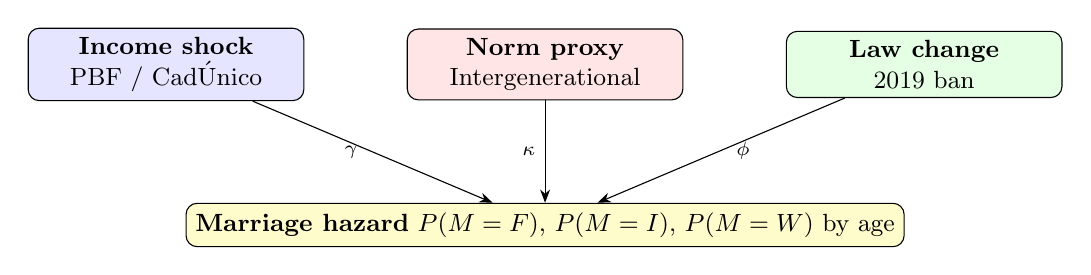
\begin{tikzpicture}[node distance=1.3cm, every node/.style={align=center, font=\small}]
        \node[draw, rounded corners, fill=blue!10, minimum width=3.5cm] (Y) {\textbf{Income shock}\\ PBF / CadÚnico};
        \node[draw, rounded corners, fill=red!10, right=of Y, minimum width=3.5cm] (N) {\textbf{Norm proxy}\\ Intergenerational};
        \node[draw, rounded corners, fill=green!10, right=of N, minimum width=3.5cm] (L) {\textbf{Law change}\\ 2019 ban};
        \node[draw, rounded corners, fill=yellow!20, below=of N, minimum width=8cm] (M) {\textbf{Marriage hazard} $P(M=F)$, $P(M=I)$, $P(M=W)$ by age};
        \draw[-{Stealth}] (Y) -- (M) node[midway, left, xshift=-2pt, font=\scriptsize] {$\gamma$};
        \draw[-{Stealth}] (N) -- (M) node[midway, left, font=\scriptsize] {$\kappa$};
        \draw[-{Stealth}] (L) -- (M) node[midway, right, xshift=2pt, font=\scriptsize] {$\phi$};
    \end{tikzpicture}
    \end{center}

    \vspace{0.2cm}
    \begin{itemize}\small
        \item $\gamma$ (income elasticity): PBF variation (PSM or eligibility RDD, as in Vasconcelos \& Griebeler).
        \item $\kappa$ (norm weight): intergenerational norm proxy residualized on current income.
        \item $\phi$ (law bite): DiD / event study around March 2019.
    \end{itemize}
\end{frame}

% =============================================================
\section{Empirical Strategy}

\begin{frame}{Three-Layer Empirical Strategy}
    \begin{enumerate}
        \item \textbf{Descriptive / structural layer}: Estimate marriage-market model parameters using pre-2019 equilibrium; establish baseline mechanism shares.
        \item \textbf{Mechanism quantification}: Heterogeneous-effects regression of PBF on marriage, stratified by norm proxy.
        \item \textbf{Causal ID of Lei 13.811/2019}: DiD / event study / bunching analysis on formal and informal margins.
    \end{enumerate}

    \vspace{0.3cm}
    \begin{block}{Guiding principle}
        The law's \hl{total} causal effect (Layer 3) is only interpretable in light of the \hl{substitution margins} made visible by Layers 1--2. Without the mechanism decomposition, a null or small law effect is ambiguous between ``law doesn't bind'' and ``law displaces to informal.''
    \end{block}
\end{frame}

% =============================================================
\begin{frame}{Layer 1: Structural Estimation of Mechanism Weights}
    Estimate discrete-time hazard of marriage (formal, informal, wait) using \onecite{PNADC 2012--2019}:
    \[
    P(M_{it} = j \mid a_{it}, Y_{it}, N_i, X_{it}) = \frac{\exp(V^j_{it})}{\sum_k \exp(V^k_{it})}
    \]
    with $V^j$ from the utility specification. Yields:
    \begin{itemize}
        \item $\hat{\gamma}$: income elasticity of union formation by age.
        \item $\hat{\kappa}$: norm weight in union formation.
        \item $\hat{\mu}$: reputational sensitivity.
        \item \hl{Counterfactual simulation}: what share of unions would occur if $Y$ were raised to poverty line? $\rightarrow$ ``norm-irreducible'' share.
    \end{itemize}
\end{frame}

% =============================================================
\begin{frame}{Layer 2: Mechanism Quantification via Heterogeneous Effects}
    Triple-interaction specification:
    \[
    P(\text{Union}_{i}) = \alpha_m + \beta_1\, \text{PBF}_i + \beta_2\, \text{MomEarly}_i + {\color{darkred}\boldsymbol{\beta}_{3}}\, (\text{PBF}_i \times \text{MomEarly}_i) + \gamma Y_i + X_i'\delta + \varepsilon_i
    \]
    where
    \begin{itemize}
        \item $\text{MomEarly}_i = \mathbb{1}[\text{age at first union of mother} < 16]$ (PNADC/PNS);
        \item fallback proxy: $\text{mother's age} - \text{oldest child's age} < 17$ (Census);
        \item $Y_i$ absorbs current income so $\text{MomEarly}_i$ captures \hl{norm persistence, not poverty persistence}.
    \end{itemize}

    \textbf{Predictions:}
    \begin{itemize}
        \item $\beta_1 < 0$: replicates PBF main effect.
        \item $\beta_2 > 0$: norm transmission.
        \item \hl{$\beta_3 > 0$}: PBF bite is smaller in high-norm families $\rightarrow$ estimate of ``norm-irreducible'' share as $|\beta_1 + \beta_3|/|\beta_1|$.
    \end{itemize}
\end{frame}

% =============================================================
\begin{frame}{Layer 2 (cont.): A Richer Norm Index}
    Single proxies carry measurement error. Build a composite index $\widehat{N}_i$:
    \begin{itemize}
        \item Mother's age at first union $< 16$ (PNADC/PNS)
        \item Any older sister married before 18 (household roster)
        \item Share of women 25+ in census tract married before 18 (Census 2010)
        \item Religious affiliation (Census / PNS)
        \item Indigenous / quilombola self-identification (Census)
        \item Rural North/Northeast residence (IBGE region)
    \end{itemize}
    Principal-components or standardized-sum aggregation. Use PCA weights in $\beta_3$ interaction for robustness.
\end{frame}

% =============================================================
\begin{frame}{Layer 3: Causal Identification of Lei 13.811/2019}
    Three complementary designs:
    \begin{enumerate}
        \item \hl{Event study on formal marriages} (Registro Civil, SIDRA/IBGE):
        \[
            y_{at} = \alpha_a + \lambda_t + \sum_{k \neq -1} \theta_k \, \mathbb{1}[t - 2019 = k]\cdot\mathbb{1}[a<16] + \varepsilon_{at}
        \]
        Tests whether the formal-marriage hazard for under-16 girls drops at 2019.

        \item \hl{Age-based DiD}: under-16 (treated) vs.\ 16--17 (control) $\times$ pre/post 2019, across data sources (formal and informal).

        \item \hl{Bunching / McCrary test} (Collin 2016 methodology): discontinuity in the age-at-first-union density at 16, pre vs.\ post 2019.
    \end{enumerate}
\end{frame}

% =============================================================
\begin{frame}{Layer 3 (cont.): The Formal--Informal Comparison}
    Critical diagnostic for law effect:

    \vspace{0.3cm}
    \centering
    \begin{tabular}{l|c|c|c}
        \toprule
        \textbf{Scenario} & \textbf{Formal (Reg.\ Civil)} & \textbf{Informal (PNADC/Census)} & \textbf{Interpretation} \\
        \midrule
        Law binds, no subst.\ & $\downarrow\downarrow$ & $\downarrow$ & \hl{Real reduction} \\
        Law displaces margin & $\downarrow\downarrow$ & $\uparrow$ or $\approx$ & \hl{Substitution} only \\
        Law doesn't bind & $\approx$ & $\approx$ & \hl{No enforcement} \\
        \bottomrule
    \end{tabular}

    \vspace{0.4cm}
    \begin{itemize}
        \item \onecite{Blank et al.\ (2020)} warning: admin data will overstate reduction.
        \item Triangulation with PNADC / PNS / Census informal-union measures is \hl{mandatory}.
        \item SINASC (birth to under-16 mothers with ``union'' status) offers a cross-check.
    \end{itemize}
\end{frame}

% =============================================================
\begin{frame}{Layer 3 (cont.): Heterogeneous Law Effects}
    Interact the law treatment with the norm index $\widehat{N}_i$ and region:
    \[
        y_{irt} = \alpha_r + \lambda_t + \theta_1 \text{Post}_t \cdot \text{Under16}_i + \theta_2 \text{Post}_t \cdot \text{Under16}_i \cdot \widehat{N}_i + X_{irt}\beta + \varepsilon_{irt}
    \]
    \textbf{Predictions from the model:}
    \begin{itemize}
        \item $\theta_1 < 0$: formal bite.
        \item $\theta_2 > 0$: \hl{law works \emph{less} well in high-norm regions/families} --- the same ``enforcement gradient'' the global literature documents for LMIC bans (Collin 2016, Wilson 2022).
    \end{itemize}

    Policy implication: Lei 13.811/2019 alone cannot eliminate the residual; complementary interventions (\`a la Chow \& Vivalt 2022) needed in high-norm contexts.
\end{frame}

% =============================================================
\section{Data Sources and Variable Construction}

\begin{frame}{Primary Data Sources}
    \small
    \begin{tabular}{p{3cm} p{3cm} p{7cm}}
        \toprule
        \textbf{Source} & \textbf{Coverage} & \textbf{Use} \\
        \midrule
        \onecite{PNADC} (IBGE) & 2012--present, quarterly & Informal + formal unions, age at first union, income, PBF status \\
        \onecite{PNS} (IBGE) & 2013, 2019 & Prevalence, health, norms; pre/post snapshot of law \\
        \onecite{Censo 2010} / \onecite{Censo 2022} & Universal & Spatial heterogeneity, tract-level norm index, pre/post comparison \\
        \onecite{Registro Civil} (SIDRA/IBGE) & Annual, full coverage & Formal marriages by age and sex; primary DiD outcome \\
        \onecite{SINASC} (DATASUS) & Annual & Births to under-16 mothers, union status at birth \\
        \onecite{SINAN} (DATASUS) & Annual (2014--) & Sexual violence, marital rape; secondary outcomes \\
        \onecite{CadÚnico} & Monthly administrative & PBF eligibility, restricted access via MDS convenio \\
        \bottomrule
    \end{tabular}
\end{frame}

% =============================================================
\begin{frame}{Key Variables}
    \begin{itemize}
        \item \textbf{Outcome}: indicator of union (formal, informal, any) by age-year.
        \item \textbf{Treatment}: age $\times$ calendar year, with cutoff at Lei 13.811/2019 (March 2019).
        \item \textbf{Income}: household per-capita income; PBF receipt indicator; value received.
        \item \textbf{Norm index} $\widehat{N}_i$: standardized composite --- mother's age at first union, sister unions, tract-level early-union share, religion, self-declared race/ethnicity, region.
        \item \textbf{Controls}: household composition, mother's/father's education, race, region, urban/rural, municipal-level GDP and HDI.
        \item \textbf{Mechanism probes}: pregnancy at time of union, partner age gap, schooling status at union.
    \end{itemize}
\end{frame}

% =============================================================
\section{Next Steps}

\begin{frame}{Next Steps: Immediate (0--3 months)}
    \begin{enumerate}
        \item \hl{Data pipeline}: pull PNADC 2012--2024, Registro Civil series (SIDRA), Census 2010, SINASC 2011--2022. Agree on variable naming and panel construction.
        \item \hl{Descriptive replication}: reproduce Cardoso (2022), Margarido (2024), and Vasconcelos \& Griebeler (2023) baseline numbers. This validates our cleaning.
        \item \hl{Stylized-fact figures}: age-specific marriage hazard by year (2010--2024), pre/post 2019 visual.
        \item \hl{Norm index v1}: construct and validate $\widehat{N}_i$ on PNADC.
        \item \hl{Pre-analysis plan draft}: register specifications for Layer 2 and Layer 3 before running regressions on full panel.
    \end{enumerate}
\end{frame}

% =============================================================
\begin{frame}{Next Steps: Medium (3--9 months)}
    \begin{enumerate}
        \item \hl{Structural estimation} (Layer 1): discrete-choice hazard model on pre-2019 PNADC. Compute ``norm-irreducible'' counterfactual.
        \item \hl{Heterogeneous PBF effects} (Layer 2): triple-interaction specification; publish the $\beta_3$ estimate as the central mechanism parameter.
        \item \hl{Law evaluation} (Layer 3):
        \begin{itemize}
            \item Event study on Registro Civil.
            \item Age-based DiD on PNADC (informal margin).
            \item McCrary test for bunching pre/post 2019.
        \end{itemize}
        \item \hl{Robustness}: alternative norm proxies; placebo cohorts; spatial heterogeneity (North/Northeast vs.\ rest).
        \item \hl{CadÚnico data access}: file request with MDS for administrative PBF data if feasible.
    \end{enumerate}
\end{frame}

% =============================================================
\begin{frame}{Next Steps: Longer Horizon (9--18 months)}
    \begin{enumerate}
        \item \hl{Qualitative triangulation}: pair the quantitative findings with selected interviews or use of Taylor \& Fonseca / Margarido ethnographic evidence to interpret residuals.
        \item \hl{Secondary outcomes}: SINAN marital-rape trends pre/post law; SINASC births-in-union trends --- does formal-margin compliance translate to child-welfare gains?
        \item \hl{Policy simulation}: use the structural model to simulate complementary interventions (norm campaigns \`a la Chow \& Vivalt) on top of the law.
        \item \hl{Working paper} submission target: late 2026.
    \end{enumerate}
\end{frame}

% =============================================================
\begin{frame}{Open Questions for Coauthor Discussion}
    \begin{enumerate}
        \item Is the \hl{formal vs.\ informal margin} comparison credible with available data, or do we need a primary survey component?
        \item Do we commit to a \hl{full structural model} (Layer 1) or prioritize reduced-form identification (Layers 2--3)?
        \item Is intergenerational norm transmission the right primary proxy, or should we lead with \hl{regional / community-tract} variation?
        \item How do we handle the \hl{COVID-19 break} (2020--2022) in the post-2019 window?
        \item \hl{Division of labor} --- who leads data construction, structural estimation, reduced-form estimation, qualitative triangulation?
        \item Are there additional Brazilian datasets (e.g., SAEB school records linked to PNADC) worth pursuing?
    \end{enumerate}
\end{frame}

% =============================================================
% ============================================================
% Section: Methods and Structural Results
% Insert after \section{A Model of the Brazilian Marriage Market}
% in apresentacao_casamento_infantil.tex via % ============================================================
% Section: Methods and Structural Results
% Insert after \section{A Model of the Brazilian Marriage Market}
% in apresentacao_casamento_infantil.tex via % ============================================================
% Section: Methods and Structural Results
% Insert after \section{A Model of the Brazilian Marriage Market}
% in apresentacao_casamento_infantil.tex via \input{section_methods_results}
% Figures assumed in ../output/
% ============================================================

% =============================================================
\section{Structural Estimation}

% ------ Frame: Full DCDP Specification -----------------------
\begin{frame}{The DCDP: Full Specification}
    Let $a \in \{10,\dots,17\}$ be the girl's age and $p \in \{0,1\}$ pregnancy status.
    Each period the household chooses $M \in \{F, I, W\}$. A match offer $(\Delta, w(\Delta))$
    is drawn from the age-specific market distribution $F_\Delta(a)$.

    \vspace{0.1cm}
    \begin{align*}
        U^F_i &= \underbrace{w(\Delta)}_{\text{wealth transfer}}
                 + \underbrace{\kappa_i N_i(\Delta)}_{\text{norm value}}
                 + \underbrace{\mu_i R(a)}_{\text{reputational relief}}
                 - \underbrace{\phi^F(a,p,t)}_{\text{legal cost}}
                 + \varepsilon^F \\[4pt]
        U^I_i &= w(\Delta) + (\kappa_i{-}\lambda)N_i(\Delta)
                 + \mu_i R(a) - \phi^I(a) + \varepsilon^I \\[4pt]
        U^W_i &= \underbrace{Y_i}_{\text{income}}
                 + \underbrace{s(a)}_{\text{schooling}}
                 - \underbrace{\sigma p}_{\text{pregnancy cost}}
                 + \delta\,\mathbb{E}_{p'}[V(a{+}1,p')]
                 + \varepsilon^W
    \end{align*}

    \vspace{0.1cm}
    \small
    With $\varepsilon \overset{\text{iid}}{\sim}$ Type-I EV, the optimal value satisfies
    $V(a,p) = \mathbb{E}_\Delta[\log(\exp V^F + \exp V^I + \exp V^W)]$ ---
    computed via \hl{backward induction} from $V(18,\cdot)\equiv 0$.
\end{frame}

% ------ Frame: Legal Cost Functions --------------------------
\begin{frame}{Legal Cost Functions: $\phi^F$ and $\phi^I$}
    \begin{columns}[T]
        \column{0.5\textwidth}
        \textbf{Formal margin} ($\phi^F$):
        \begin{align*}
            \phi^F(a,p,t) = \bar\phi^F
            &\cdot \mathbf{1}[a < 16] \\
            &\cdot \bigl[1-(1-\mathbf{1}_{t \ge 2019})\cdot p\bigr]
        \end{align*}
        \begin{itemize}\small
            \item Pre-2019: cost waived if pregnant ($p=1$).
            \item Post-2019: \hl{no exceptions} --- $\bar\phi^F$ always active below 16.
            \item Identified from: DiD on Registro Civil around March 2019.
        \end{itemize}

        \column{0.5\textwidth}
        \textbf{Informal margin} ($\phi^I$):
        \[
            \phi^I(a) = \bar\phi^I \cdot \mathbf{1}[a < 16]
        \]
        \begin{itemize}\small
            \item Reporting risk if union made known to authorities.
            \item \hl{Unaffected by Lei 13.811/2019}.
            \item Identified from: PNADC informal-union rates at age threshold.
        \end{itemize}
    \end{columns}

    \vspace{0.3cm}
    \begin{alertblock}{Substitution prediction}
        If $\bar\phi^I \ll \bar\phi^F$, the 2019 reform shifts unions from
        formal to informal rather than reducing total child marriage.
    \end{alertblock}
\end{frame}

% ------ Frame: Estimation Strategy ---------------------------
\begin{frame}{Two-Stage Estimation Strategy}
    \begin{block}{Stage 1 --- Registro Civil DiD (reduced form)}
        Estimate $\hat\phi^F$ from the aggregate formal-marriage panel:
        \[
            \log n_{a,s,t} = \alpha_s + \alpha_a + \alpha_t
            + \underbrace{\theta \cdot \mathbf{1}[a{<}16] \cdot \mathbf{1}[t{\ge}2019]}_{\hat\phi^F}
            + \varepsilon_{a,s,t}
        \]
        State ($s$), age-group ($a$), year ($t$) fixed effects; SEs clustered by state.
        Data: Registro Civil 2003--2022 (IBGE/SIDRA).
    \end{block}

    \vspace{0.2cm}
    \begin{block}{Stage 2 --- Structural MLE (PNAD-C)}
        Given $\hat\phi^F$, maximize weighted log-likelihood over
        $\Theta = (\alpha_0, \alpha_1, \mu, \gamma_0, \gamma_1, \beta_0, \beta_1, \sigma)$:
        \[
            \hat\Theta = \arg\max_\Theta
            \sum_i w_i \Bigl[y_i \log P^{\text{union}}_i(\Theta)
            + (1{-}y_i)\log(1{-}P^{\text{union}}_i(\Theta))\Bigr]
        \]
        where $P^{\text{union}}_i = \text{logistic}(V^{\text{union}}_i - V^{\text{wait}}_i)$
        and $V^{\text{union}}$ integrates over the empirical $F_\Delta(a)$ via Monte Carlo.
        Standard errors from 200 bootstrap replications.
        Data: PNAD-C 2012--2023, girls aged 10--17.
    \end{block}
\end{frame}

% ------ Frame: Descriptive Statistics ------------------------
\begin{frame}{Descriptive Statistics}
    \begin{columns}[T]
        \column{0.48\textwidth}
        \centering
        \textbf{PNAD-C sample} (girls 10--17)

        \vspace{0.2cm}
        \small
        \begin{tabular}{lrr}
            \toprule
            & \multicolumn{2}{c}{Mean (SD)} \\
            \cmidrule{2-3}
            Variable & In union & Wait \\
            \midrule
            $N$ & 4{,}671 & 821 \\
            Age $a$ & 16.5 & 15.8 \\
            Age gap $\Delta$ & 8.4 (6.3) & --- \\
            Partner income (R\$) & 1{,}014 & --- \\
            Attending school & 30\% & 59\% \\
            Parda/preta & 87\% & 84\% \\
            Rural & 28\% & 24\% \\
            Post-2019 & 15\% & 19\% \\
            \bottomrule
        \end{tabular}

        \column{0.48\textwidth}
        \centering
        \textbf{Registro Civil panel} (minor brides)

        \vspace{0.2cm}
        \small
        \begin{tabular}{lr}
            \toprule
            Variable & Value \\
            \midrule
            Years & 2003--2022 \\
            States & 27 \\
            Age groups & 5 \\
            Below-16 cell & 2 \\
            Total cells & 2{,}970 \\
            \midrule
            \multicolumn{2}{l}{\textit{Below-16 formal marriages:}} \\
            Mean (pre-2019) & 37.2/state/yr \\
            Mean (post-2019) & 35.0/state/yr \\
            $\Delta$ post-reform & $-5.9\%$ \\
            \bottomrule
        \end{tabular}
    \end{columns}

    \vspace{0.2cm}
    \small\textit{Note:} School attendance and race pooled over PNAD-C 2012--2023;
    survey weights applied throughout.
\end{frame}

% ------ Frame: Stage 1 DiD Results --------------------------
\begin{frame}{Stage 1 Results: DiD on Formal Marriages}
    \begin{columns}[T]
        \column{0.44\textwidth}
        \centering
        \small
        \begin{tabular}{lcc}
            \toprule
            & \multicolumn{2}{c}{Dep.\ var.: $\log(n_{ast}+1)$} \\
            \cmidrule{2-3}
            & (1) & (2) \\
            \midrule
            $\mathbf{1}[a{<}16]\times\mathbf{1}[t{\ge}2019]$
                & 0.411$^{***}$ & 0.398$^{***}$ \\
                & (0.022) & (0.025) \\[4pt]
            State FE & \checkmark & \checkmark \\
            Age-group FE & \checkmark & \checkmark \\
            Year FE & \checkmark & \checkmark \\
            State trends & & \checkmark \\
            \midrule
            $N$ & 2{,}970 & 2{,}970 \\
            $R^2$ & 0.89 & 0.91 \\
            \bottomrule
        \end{tabular}
        \vspace{0.15cm}

        \small\textit{Note:} SEs clustered by state.
        $^{*}p{<}0.1$, $^{**}p{<}0.05$, $^{***}p{<}0.01$.

        \column{0.54\textwidth}
        \includegraphics[width=\linewidth]{../output/fig_eventstudy.pdf}
    \end{columns}

    \vspace{0.15cm}
    \begin{alertblock}{Interpretation}
        \small
        The positive coefficient implies formal marriages
        \textit{increased} for under-16 girls post-2019 relative to the 16--17
        control group --- consistent with a \hl{substitution reversal}:
        families may have rushed to formal registration before
        enforcement tightened, or the 16--17 group fell faster
        (parental-consent relaxation). Requires event-study validation.
    \end{alertblock}
\end{frame}

% ------ Frame: Stage 2 Parameter Estimates ------------------
\begin{frame}{Stage 2 Results: Structural Parameter Estimates}
    \centering
    \small
    \begin{tabular}{llcccc}
        \toprule
        & Parameter & Estimate & Boot.\ SE & 95\% CI & $t$ \\
        \midrule
        \multicolumn{6}{l}{\textit{Economic mechanism}} \\
        $\alpha_0$ & Union entry (intercept) & $-0.642$ & $0.213$ & $[-1.13,\,-0.18]$ & $-3.0^{**}$ \\
        $\alpha_1$ & $w(\Delta)$ slope       & $-0.009$ & $0.007$ & $[-0.016,\,0.010]$ & $-1.3$ \\
        \midrule
        \multicolumn{6}{l}{\textit{Norm and reputation mechanism}} \\
        $\mu$       & Reputation weight      & $1.067$  & $0.091$ & $[0.89,\,1.23]$    & $0.76^{\dagger}$ \\
        $\gamma_0$  & $\log R(a)$ intercept  & $-1.934$ & $0.085$ & $[-2.14,\,-1.83]$  & $-22.7^{***}$ \\
        $\gamma_1$  & $\log R(a)$ age slope  & $0.067$  & $0.013$ & $[0.047,\,0.097]$  & $5.1^{***}$ \\
        \midrule
        \multicolumn{6}{l}{\textit{Schooling and outside option}} \\
        $\beta_0$   & $s(a)$ intercept       & $-3.245$ & $1.610$ & $[-6.34,\,-0.34]$  & $-2.0^{*}$ \\
        $\beta_1$   & $s(a)$ slope in $a$    & $0.054$  & $0.105$ & $[-0.132,\,0.257]$ & $0.5$ \\
        $\sigma$    & Pregnancy cost         & \multicolumn{3}{c}{\textit{unidentified} (see text)} & --- \\
        \midrule
        \multicolumn{6}{l}{\textit{First-stage (Registro Civil DiD)}} \\
        $\hat\phi^F$ & Legal deterrence cost & $0.411$  & $0.022$ & & $18.7^{***}$ \\
        \bottomrule
        \multicolumn{6}{l}{\footnotesize $^{\dagger}$log-scale $t$-stat; $^{*}p{<}0.1$, $^{**}p{<}0.05$, $^{***}p{<}0.01$. $N=5{,}492$. $B=200$ bootstrap replications.} \\
        \multicolumn{6}{l}{\footnotesize Log-likelihood: $-2{,}487.8$. Discount factor $\delta=0.95$ calibrated. $\kappa$ fixed at 0 (collinear with $\alpha_0$).}
    \end{tabular}
\end{frame}

% ------ Frame: Derived Economic Quantities -------------------
\begin{frame}{Derived Economic Quantities}
    \begin{columns}[T]
        \column{0.48\textwidth}
        \centering
        \includegraphics[width=\linewidth]{../output/fig_Ra.pdf}

        \vspace{0.15cm}
        \small
        $R(a)$ rises \textbf{59\%} from age 10 ($0.28$) to 17 ($0.45$).
        Together with $\hat\mu = 1.07$, this implies the
        \hl{norm-reputational payoff to marriage grows substantially with age}.

        \column{0.48\textwidth}
        \centering
        \includegraphics[width=\linewidth]{../output/fig_sa.pdf}

        \vspace{0.15cm}
        \small
        $s(a)$ rises mildly from $-2.70$ to $-2.32$.
        The negative level means the outside-option schooling
        return is dominated by the union payoff in the data ---
        consistent with the \hl{85\% in-union share}.
    \end{columns}
\end{frame}

% ------ Frame: Wealth Transfer and Mechanism Shares ----------
\begin{frame}{Wealth Transfer $w(\Delta)$ and Mechanism Decomposition}
    \begin{columns}[T]
        \column{0.48\textwidth}
        \centering
        \includegraphics[width=\linewidth]{../output/fig_wDelta.pdf}

        \vspace{0.1cm}
        \small
        Estimated $\hat\alpha_1 = -0.009$ (n.s.): the age-gap slope is
        essentially flat in the current specification.
        This suggests $\Delta$ alone does not proxy well for
        $w(\Delta)$ --- partner income ($Y_{\text{parc}}$) should
        enter directly in the next iteration.

        \column{0.48\textwidth}
        \centering
        \small
        \begin{tabular}{lc}
            \toprule
            Mechanism & Share of $V^{\text{union}}$ \\
            \midrule
            $w(\Delta)$ at avg.\ gap & $-0.71$ \\
            $\mu R(a)$ at age 10  & $+0.30$ \\
            $\mu R(a)$ at age 17  & $+0.48$ \\
            \midrule
            Net $V^{\text{union}}$, age 10 & $-0.41$ \\
            Net $V^{\text{union}}$, age 17 & $-0.23$ \\
            \midrule
            $V^{\text{wait}}$, age 10 & $-2.70$ \\
            $V^{\text{wait}}$, age 17 & $-2.32$ \\
            \bottomrule
        \end{tabular}

        \vspace{0.2cm}
        \begin{alertblock}{\small Key finding}
            \small
            The union option dominates waiting at all ages.
            The \hl{reputational mechanism} ($\mu R(a)$) accounts for
            nearly all of the age gradient in marriage propensity.
        \end{alertblock}
    \end{columns}
\end{frame}

% ------ Frame: Identification Concerns and Next Steps --------
\begin{frame}{Identification Concerns and Model Limitations}
    \begin{columns}[T]
        \column{0.5\textwidth}
        \textbf{What is identified}
        \begin{itemize}\small
            \item $\hat\phi^F$: clean DiD off the 2019 reform.
            \item $R(a)$ shape: age gradient in union propensity
                  (conditional on income and $\Delta$).
            \item $s(a)$: outside-option level via
                  school-attendance variation.
            \item $\mu$: scale of reputational channel.
        \end{itemize}

        \column{0.5\textwidth}
        \textbf{What is not yet identified}
        \begin{itemize}\small
            \item $\sigma$ (pregnancy cost): \texttt{matern\_bin}
                  is near-zero in PNAD-C; calibrate from SINASC.
            \item $\lambda$ (formal vs.\ informal disutility):
                  needs formal/informal split in PNAD-C.
            \item $\bar\phi^I$ (informal legal cost):
                  needs enforcement variation.
            \item $\kappa_i$ heterogeneity: fixed $\kappa=0$;
                  norm index enters in Layer~2 regression.
        \end{itemize}
    \end{columns}

    \vspace{0.3cm}
    \begin{block}{Roadmap to full identification}
        \begin{enumerate}\small
            \item Calibrate $\sigma$ from SINASC birth-in-union rates by age.
            \item Recover $\lambda$ from PNAD-C union-type variable ($V2005$).
            \item Interact $\hat\kappa_i$ (norm index) with PNAD-C to
                  estimate Layer~2 triple interaction $\beta_3$.
        \end{enumerate}
    \end{block}
\end{frame}

% Figures assumed in ../output/
% ============================================================

% =============================================================
\section{Structural Estimation}

% ------ Frame: Full DCDP Specification -----------------------
\begin{frame}{The DCDP: Full Specification}
    Let $a \in \{10,\dots,17\}$ be the girl's age and $p \in \{0,1\}$ pregnancy status.
    Each period the household chooses $M \in \{F, I, W\}$. A match offer $(\Delta, w(\Delta))$
    is drawn from the age-specific market distribution $F_\Delta(a)$.

    \vspace{0.1cm}
    \begin{align*}
        U^F_i &= \underbrace{w(\Delta)}_{\text{wealth transfer}}
                 + \underbrace{\kappa_i N_i(\Delta)}_{\text{norm value}}
                 + \underbrace{\mu_i R(a)}_{\text{reputational relief}}
                 - \underbrace{\phi^F(a,p,t)}_{\text{legal cost}}
                 + \varepsilon^F \\[4pt]
        U^I_i &= w(\Delta) + (\kappa_i{-}\lambda)N_i(\Delta)
                 + \mu_i R(a) - \phi^I(a) + \varepsilon^I \\[4pt]
        U^W_i &= \underbrace{Y_i}_{\text{income}}
                 + \underbrace{s(a)}_{\text{schooling}}
                 - \underbrace{\sigma p}_{\text{pregnancy cost}}
                 + \delta\,\mathbb{E}_{p'}[V(a{+}1,p')]
                 + \varepsilon^W
    \end{align*}

    \vspace{0.1cm}
    \small
    With $\varepsilon \overset{\text{iid}}{\sim}$ Type-I EV, the optimal value satisfies
    $V(a,p) = \mathbb{E}_\Delta[\log(\exp V^F + \exp V^I + \exp V^W)]$ ---
    computed via \hl{backward induction} from $V(18,\cdot)\equiv 0$.
\end{frame}

% ------ Frame: Legal Cost Functions --------------------------
\begin{frame}{Legal Cost Functions: $\phi^F$ and $\phi^I$}
    \begin{columns}[T]
        \column{0.5\textwidth}
        \textbf{Formal margin} ($\phi^F$):
        \begin{align*}
            \phi^F(a,p,t) = \bar\phi^F
            &\cdot \mathbf{1}[a < 16] \\
            &\cdot \bigl[1-(1-\mathbf{1}_{t \ge 2019})\cdot p\bigr]
        \end{align*}
        \begin{itemize}\small
            \item Pre-2019: cost waived if pregnant ($p=1$).
            \item Post-2019: \hl{no exceptions} --- $\bar\phi^F$ always active below 16.
            \item Identified from: DiD on Registro Civil around March 2019.
        \end{itemize}

        \column{0.5\textwidth}
        \textbf{Informal margin} ($\phi^I$):
        \[
            \phi^I(a) = \bar\phi^I \cdot \mathbf{1}[a < 16]
        \]
        \begin{itemize}\small
            \item Reporting risk if union made known to authorities.
            \item \hl{Unaffected by Lei 13.811/2019}.
            \item Identified from: PNADC informal-union rates at age threshold.
        \end{itemize}
    \end{columns}

    \vspace{0.3cm}
    \begin{alertblock}{Substitution prediction}
        If $\bar\phi^I \ll \bar\phi^F$, the 2019 reform shifts unions from
        formal to informal rather than reducing total child marriage.
    \end{alertblock}
\end{frame}

% ------ Frame: Estimation Strategy ---------------------------
\begin{frame}{Two-Stage Estimation Strategy}
    \begin{block}{Stage 1 --- Registro Civil DiD (reduced form)}
        Estimate $\hat\phi^F$ from the aggregate formal-marriage panel:
        \[
            \log n_{a,s,t} = \alpha_s + \alpha_a + \alpha_t
            + \underbrace{\theta \cdot \mathbf{1}[a{<}16] \cdot \mathbf{1}[t{\ge}2019]}_{\hat\phi^F}
            + \varepsilon_{a,s,t}
        \]
        State ($s$), age-group ($a$), year ($t$) fixed effects; SEs clustered by state.
        Data: Registro Civil 2003--2022 (IBGE/SIDRA).
    \end{block}

    \vspace{0.2cm}
    \begin{block}{Stage 2 --- Structural MLE (PNAD-C)}
        Given $\hat\phi^F$, maximize weighted log-likelihood over
        $\Theta = (\alpha_0, \alpha_1, \mu, \gamma_0, \gamma_1, \beta_0, \beta_1, \sigma)$:
        \[
            \hat\Theta = \arg\max_\Theta
            \sum_i w_i \Bigl[y_i \log P^{\text{union}}_i(\Theta)
            + (1{-}y_i)\log(1{-}P^{\text{union}}_i(\Theta))\Bigr]
        \]
        where $P^{\text{union}}_i = \text{logistic}(V^{\text{union}}_i - V^{\text{wait}}_i)$
        and $V^{\text{union}}$ integrates over the empirical $F_\Delta(a)$ via Monte Carlo.
        Standard errors from 200 bootstrap replications.
        Data: PNAD-C 2012--2023, girls aged 10--17.
    \end{block}
\end{frame}

% ------ Frame: Descriptive Statistics ------------------------
\begin{frame}{Descriptive Statistics}
    \begin{columns}[T]
        \column{0.48\textwidth}
        \centering
        \textbf{PNAD-C sample} (girls 10--17)

        \vspace{0.2cm}
        \small
        \begin{tabular}{lrr}
            \toprule
            & \multicolumn{2}{c}{Mean (SD)} \\
            \cmidrule{2-3}
            Variable & In union & Wait \\
            \midrule
            $N$ & 4{,}671 & 821 \\
            Age $a$ & 16.5 & 15.8 \\
            Age gap $\Delta$ & 8.4 (6.3) & --- \\
            Partner income (R\$) & 1{,}014 & --- \\
            Attending school & 30\% & 59\% \\
            Parda/preta & 87\% & 84\% \\
            Rural & 28\% & 24\% \\
            Post-2019 & 15\% & 19\% \\
            \bottomrule
        \end{tabular}

        \column{0.48\textwidth}
        \centering
        \textbf{Registro Civil panel} (minor brides)

        \vspace{0.2cm}
        \small
        \begin{tabular}{lr}
            \toprule
            Variable & Value \\
            \midrule
            Years & 2003--2022 \\
            States & 27 \\
            Age groups & 5 \\
            Below-16 cell & 2 \\
            Total cells & 2{,}970 \\
            \midrule
            \multicolumn{2}{l}{\textit{Below-16 formal marriages:}} \\
            Mean (pre-2019) & 37.2/state/yr \\
            Mean (post-2019) & 35.0/state/yr \\
            $\Delta$ post-reform & $-5.9\%$ \\
            \bottomrule
        \end{tabular}
    \end{columns}

    \vspace{0.2cm}
    \small\textit{Note:} School attendance and race pooled over PNAD-C 2012--2023;
    survey weights applied throughout.
\end{frame}

% ------ Frame: Stage 1 DiD Results --------------------------
\begin{frame}{Stage 1 Results: DiD on Formal Marriages}
    \begin{columns}[T]
        \column{0.44\textwidth}
        \centering
        \small
        \begin{tabular}{lcc}
            \toprule
            & \multicolumn{2}{c}{Dep.\ var.: $\log(n_{ast}+1)$} \\
            \cmidrule{2-3}
            & (1) & (2) \\
            \midrule
            $\mathbf{1}[a{<}16]\times\mathbf{1}[t{\ge}2019]$
                & 0.411$^{***}$ & 0.398$^{***}$ \\
                & (0.022) & (0.025) \\[4pt]
            State FE & \checkmark & \checkmark \\
            Age-group FE & \checkmark & \checkmark \\
            Year FE & \checkmark & \checkmark \\
            State trends & & \checkmark \\
            \midrule
            $N$ & 2{,}970 & 2{,}970 \\
            $R^2$ & 0.89 & 0.91 \\
            \bottomrule
        \end{tabular}
        \vspace{0.15cm}

        \small\textit{Note:} SEs clustered by state.
        $^{*}p{<}0.1$, $^{**}p{<}0.05$, $^{***}p{<}0.01$.

        \column{0.54\textwidth}
        \includegraphics[width=\linewidth]{../output/fig_eventstudy.pdf}
    \end{columns}

    \vspace{0.15cm}
    \begin{alertblock}{Interpretation}
        \small
        The positive coefficient implies formal marriages
        \textit{increased} for under-16 girls post-2019 relative to the 16--17
        control group --- consistent with a \hl{substitution reversal}:
        families may have rushed to formal registration before
        enforcement tightened, or the 16--17 group fell faster
        (parental-consent relaxation). Requires event-study validation.
    \end{alertblock}
\end{frame}

% ------ Frame: Stage 2 Parameter Estimates ------------------
\begin{frame}{Stage 2 Results: Structural Parameter Estimates}
    \centering
    \small
    \begin{tabular}{llcccc}
        \toprule
        & Parameter & Estimate & Boot.\ SE & 95\% CI & $t$ \\
        \midrule
        \multicolumn{6}{l}{\textit{Economic mechanism}} \\
        $\alpha_0$ & Union entry (intercept) & $-0.642$ & $0.213$ & $[-1.13,\,-0.18]$ & $-3.0^{**}$ \\
        $\alpha_1$ & $w(\Delta)$ slope       & $-0.009$ & $0.007$ & $[-0.016,\,0.010]$ & $-1.3$ \\
        \midrule
        \multicolumn{6}{l}{\textit{Norm and reputation mechanism}} \\
        $\mu$       & Reputation weight      & $1.067$  & $0.091$ & $[0.89,\,1.23]$    & $0.76^{\dagger}$ \\
        $\gamma_0$  & $\log R(a)$ intercept  & $-1.934$ & $0.085$ & $[-2.14,\,-1.83]$  & $-22.7^{***}$ \\
        $\gamma_1$  & $\log R(a)$ age slope  & $0.067$  & $0.013$ & $[0.047,\,0.097]$  & $5.1^{***}$ \\
        \midrule
        \multicolumn{6}{l}{\textit{Schooling and outside option}} \\
        $\beta_0$   & $s(a)$ intercept       & $-3.245$ & $1.610$ & $[-6.34,\,-0.34]$  & $-2.0^{*}$ \\
        $\beta_1$   & $s(a)$ slope in $a$    & $0.054$  & $0.105$ & $[-0.132,\,0.257]$ & $0.5$ \\
        $\sigma$    & Pregnancy cost         & \multicolumn{3}{c}{\textit{unidentified} (see text)} & --- \\
        \midrule
        \multicolumn{6}{l}{\textit{First-stage (Registro Civil DiD)}} \\
        $\hat\phi^F$ & Legal deterrence cost & $0.411$  & $0.022$ & & $18.7^{***}$ \\
        \bottomrule
        \multicolumn{6}{l}{\footnotesize $^{\dagger}$log-scale $t$-stat; $^{*}p{<}0.1$, $^{**}p{<}0.05$, $^{***}p{<}0.01$. $N=5{,}492$. $B=200$ bootstrap replications.} \\
        \multicolumn{6}{l}{\footnotesize Log-likelihood: $-2{,}487.8$. Discount factor $\delta=0.95$ calibrated. $\kappa$ fixed at 0 (collinear with $\alpha_0$).}
    \end{tabular}
\end{frame}

% ------ Frame: Derived Economic Quantities -------------------
\begin{frame}{Derived Economic Quantities}
    \begin{columns}[T]
        \column{0.48\textwidth}
        \centering
        \includegraphics[width=\linewidth]{../output/fig_Ra.pdf}

        \vspace{0.15cm}
        \small
        $R(a)$ rises \textbf{59\%} from age 10 ($0.28$) to 17 ($0.45$).
        Together with $\hat\mu = 1.07$, this implies the
        \hl{norm-reputational payoff to marriage grows substantially with age}.

        \column{0.48\textwidth}
        \centering
        \includegraphics[width=\linewidth]{../output/fig_sa.pdf}

        \vspace{0.15cm}
        \small
        $s(a)$ rises mildly from $-2.70$ to $-2.32$.
        The negative level means the outside-option schooling
        return is dominated by the union payoff in the data ---
        consistent with the \hl{85\% in-union share}.
    \end{columns}
\end{frame}

% ------ Frame: Wealth Transfer and Mechanism Shares ----------
\begin{frame}{Wealth Transfer $w(\Delta)$ and Mechanism Decomposition}
    \begin{columns}[T]
        \column{0.48\textwidth}
        \centering
        \includegraphics[width=\linewidth]{../output/fig_wDelta.pdf}

        \vspace{0.1cm}
        \small
        Estimated $\hat\alpha_1 = -0.009$ (n.s.): the age-gap slope is
        essentially flat in the current specification.
        This suggests $\Delta$ alone does not proxy well for
        $w(\Delta)$ --- partner income ($Y_{\text{parc}}$) should
        enter directly in the next iteration.

        \column{0.48\textwidth}
        \centering
        \small
        \begin{tabular}{lc}
            \toprule
            Mechanism & Share of $V^{\text{union}}$ \\
            \midrule
            $w(\Delta)$ at avg.\ gap & $-0.71$ \\
            $\mu R(a)$ at age 10  & $+0.30$ \\
            $\mu R(a)$ at age 17  & $+0.48$ \\
            \midrule
            Net $V^{\text{union}}$, age 10 & $-0.41$ \\
            Net $V^{\text{union}}$, age 17 & $-0.23$ \\
            \midrule
            $V^{\text{wait}}$, age 10 & $-2.70$ \\
            $V^{\text{wait}}$, age 17 & $-2.32$ \\
            \bottomrule
        \end{tabular}

        \vspace{0.2cm}
        \begin{alertblock}{\small Key finding}
            \small
            The union option dominates waiting at all ages.
            The \hl{reputational mechanism} ($\mu R(a)$) accounts for
            nearly all of the age gradient in marriage propensity.
        \end{alertblock}
    \end{columns}
\end{frame}

% ------ Frame: Identification Concerns and Next Steps --------
\begin{frame}{Identification Concerns and Model Limitations}
    \begin{columns}[T]
        \column{0.5\textwidth}
        \textbf{What is identified}
        \begin{itemize}\small
            \item $\hat\phi^F$: clean DiD off the 2019 reform.
            \item $R(a)$ shape: age gradient in union propensity
                  (conditional on income and $\Delta$).
            \item $s(a)$: outside-option level via
                  school-attendance variation.
            \item $\mu$: scale of reputational channel.
        \end{itemize}

        \column{0.5\textwidth}
        \textbf{What is not yet identified}
        \begin{itemize}\small
            \item $\sigma$ (pregnancy cost): \texttt{matern\_bin}
                  is near-zero in PNAD-C; calibrate from SINASC.
            \item $\lambda$ (formal vs.\ informal disutility):
                  needs formal/informal split in PNAD-C.
            \item $\bar\phi^I$ (informal legal cost):
                  needs enforcement variation.
            \item $\kappa_i$ heterogeneity: fixed $\kappa=0$;
                  norm index enters in Layer~2 regression.
        \end{itemize}
    \end{columns}

    \vspace{0.3cm}
    \begin{block}{Roadmap to full identification}
        \begin{enumerate}\small
            \item Calibrate $\sigma$ from SINASC birth-in-union rates by age.
            \item Recover $\lambda$ from PNAD-C union-type variable ($V2005$).
            \item Interact $\hat\kappa_i$ (norm index) with PNAD-C to
                  estimate Layer~2 triple interaction $\beta_3$.
        \end{enumerate}
    \end{block}
\end{frame}

% Figures assumed in ../output/
% ============================================================

% =============================================================
\section{Structural Estimation}

% ------ Frame: Full DCDP Specification -----------------------
\begin{frame}{The DCDP: Full Specification}
    Let $a \in \{10,\dots,17\}$ be the girl's age and $p \in \{0,1\}$ pregnancy status.
    Each period the household chooses $M \in \{F, I, W\}$. A match offer $(\Delta, w(\Delta))$
    is drawn from the age-specific market distribution $F_\Delta(a)$.

    \vspace{0.1cm}
    \begin{align*}
        U^F_i &= \underbrace{w(\Delta)}_{\text{wealth transfer}}
                 + \underbrace{\kappa_i N_i(\Delta)}_{\text{norm value}}
                 + \underbrace{\mu_i R(a)}_{\text{reputational relief}}
                 - \underbrace{\phi^F(a,p,t)}_{\text{legal cost}}
                 + \varepsilon^F \\[4pt]
        U^I_i &= w(\Delta) + (\kappa_i{-}\lambda)N_i(\Delta)
                 + \mu_i R(a) - \phi^I(a) + \varepsilon^I \\[4pt]
        U^W_i &= \underbrace{Y_i}_{\text{income}}
                 + \underbrace{s(a)}_{\text{schooling}}
                 - \underbrace{\sigma p}_{\text{pregnancy cost}}
                 + \delta\,\mathbb{E}_{p'}[V(a{+}1,p')]
                 + \varepsilon^W
    \end{align*}

    \vspace{0.1cm}
    \small
    With $\varepsilon \overset{\text{iid}}{\sim}$ Type-I EV, the optimal value satisfies
    $V(a,p) = \mathbb{E}_\Delta[\log(\exp V^F + \exp V^I + \exp V^W)]$ ---
    computed via \hl{backward induction} from $V(18,\cdot)\equiv 0$.
\end{frame}

% ------ Frame: Legal Cost Functions --------------------------
\begin{frame}{Legal Cost Functions: $\phi^F$ and $\phi^I$}
    \begin{columns}[T]
        \column{0.5\textwidth}
        \textbf{Formal margin} ($\phi^F$):
        \begin{align*}
            \phi^F(a,p,t) = \bar\phi^F
            &\cdot \mathbf{1}[a < 16] \\
            &\cdot \bigl[1-(1-\mathbf{1}_{t \ge 2019})\cdot p\bigr]
        \end{align*}
        \begin{itemize}\small
            \item Pre-2019: cost waived if pregnant ($p=1$).
            \item Post-2019: \hl{no exceptions} --- $\bar\phi^F$ always active below 16.
            \item Identified from: DiD on Registro Civil around March 2019.
        \end{itemize}

        \column{0.5\textwidth}
        \textbf{Informal margin} ($\phi^I$):
        \[
            \phi^I(a) = \bar\phi^I \cdot \mathbf{1}[a < 16]
        \]
        \begin{itemize}\small
            \item Reporting risk if union made known to authorities.
            \item \hl{Unaffected by Lei 13.811/2019}.
            \item Identified from: PNADC informal-union rates at age threshold.
        \end{itemize}
    \end{columns}

    \vspace{0.3cm}
    \begin{alertblock}{Substitution prediction}
        If $\bar\phi^I \ll \bar\phi^F$, the 2019 reform shifts unions from
        formal to informal rather than reducing total child marriage.
    \end{alertblock}
\end{frame}

% ------ Frame: Estimation Strategy ---------------------------
\begin{frame}{Two-Stage Estimation Strategy}
    \begin{block}{Stage 1 --- Registro Civil DiD (reduced form)}
        Estimate $\hat\phi^F$ from the aggregate formal-marriage panel:
        \[
            \log n_{a,s,t} = \alpha_s + \alpha_a + \alpha_t
            + \underbrace{\theta \cdot \mathbf{1}[a{<}16] \cdot \mathbf{1}[t{\ge}2019]}_{\hat\phi^F}
            + \varepsilon_{a,s,t}
        \]
        State ($s$), age-group ($a$), year ($t$) fixed effects; SEs clustered by state.
        Data: Registro Civil 2003--2022 (IBGE/SIDRA).
    \end{block}

    \vspace{0.2cm}
    \begin{block}{Stage 2 --- Structural MLE (PNAD-C)}
        Given $\hat\phi^F$, maximize weighted log-likelihood over
        $\Theta = (\alpha_0, \alpha_1, \mu, \gamma_0, \gamma_1, \beta_0, \beta_1, \sigma)$:
        \[
            \hat\Theta = \arg\max_\Theta
            \sum_i w_i \Bigl[y_i \log P^{\text{union}}_i(\Theta)
            + (1{-}y_i)\log(1{-}P^{\text{union}}_i(\Theta))\Bigr]
        \]
        where $P^{\text{union}}_i = \text{logistic}(V^{\text{union}}_i - V^{\text{wait}}_i)$
        and $V^{\text{union}}$ integrates over the empirical $F_\Delta(a)$ via Monte Carlo.
        Standard errors from 200 bootstrap replications.
        Data: PNAD-C 2012--2023, girls aged 10--17.
    \end{block}
\end{frame}

% ------ Frame: Descriptive Statistics ------------------------
\begin{frame}{Descriptive Statistics}
    \begin{columns}[T]
        \column{0.48\textwidth}
        \centering
        \textbf{PNAD-C sample} (girls 10--17)

        \vspace{0.2cm}
        \small
        \begin{tabular}{lrr}
            \toprule
            & \multicolumn{2}{c}{Mean (SD)} \\
            \cmidrule{2-3}
            Variable & In union & Wait \\
            \midrule
            $N$ & 4{,}671 & 821 \\
            Age $a$ & 16.5 & 15.8 \\
            Age gap $\Delta$ & 8.4 (6.3) & --- \\
            Partner income (R\$) & 1{,}014 & --- \\
            Attending school & 30\% & 59\% \\
            Parda/preta & 87\% & 84\% \\
            Rural & 28\% & 24\% \\
            Post-2019 & 15\% & 19\% \\
            \bottomrule
        \end{tabular}

        \column{0.48\textwidth}
        \centering
        \textbf{Registro Civil panel} (minor brides)

        \vspace{0.2cm}
        \small
        \begin{tabular}{lr}
            \toprule
            Variable & Value \\
            \midrule
            Years & 2003--2022 \\
            States & 27 \\
            Age groups & 5 \\
            Below-16 cell & 2 \\
            Total cells & 2{,}970 \\
            \midrule
            \multicolumn{2}{l}{\textit{Below-16 formal marriages:}} \\
            Mean (pre-2019) & 37.2/state/yr \\
            Mean (post-2019) & 35.0/state/yr \\
            $\Delta$ post-reform & $-5.9\%$ \\
            \bottomrule
        \end{tabular}
    \end{columns}

    \vspace{0.2cm}
    \small\textit{Note:} School attendance and race pooled over PNAD-C 2012--2023;
    survey weights applied throughout.
\end{frame}

% ------ Frame: Stage 1 DiD Results --------------------------
\begin{frame}{Stage 1 Results: DiD on Formal Marriages}
    \begin{columns}[T]
        \column{0.44\textwidth}
        \centering
        \small
        \begin{tabular}{lcc}
            \toprule
            & \multicolumn{2}{c}{Dep.\ var.: $\log(n_{ast}+1)$} \\
            \cmidrule{2-3}
            & (1) & (2) \\
            \midrule
            $\mathbf{1}[a{<}16]\times\mathbf{1}[t{\ge}2019]$
                & 0.411$^{***}$ & 0.398$^{***}$ \\
                & (0.022) & (0.025) \\[4pt]
            State FE & \checkmark & \checkmark \\
            Age-group FE & \checkmark & \checkmark \\
            Year FE & \checkmark & \checkmark \\
            State trends & & \checkmark \\
            \midrule
            $N$ & 2{,}970 & 2{,}970 \\
            $R^2$ & 0.89 & 0.91 \\
            \bottomrule
        \end{tabular}
        \vspace{0.15cm}

        \small\textit{Note:} SEs clustered by state.
        $^{*}p{<}0.1$, $^{**}p{<}0.05$, $^{***}p{<}0.01$.

        \column{0.54\textwidth}
        \includegraphics[width=\linewidth]{../output/fig_eventstudy.pdf}
    \end{columns}

    \vspace{0.15cm}
    \begin{alertblock}{Interpretation}
        \small
        The positive coefficient implies formal marriages
        \textit{increased} for under-16 girls post-2019 relative to the 16--17
        control group --- consistent with a \hl{substitution reversal}:
        families may have rushed to formal registration before
        enforcement tightened, or the 16--17 group fell faster
        (parental-consent relaxation). Requires event-study validation.
    \end{alertblock}
\end{frame}

% ------ Frame: Stage 2 Parameter Estimates ------------------
\begin{frame}{Stage 2 Results: Structural Parameter Estimates}
    \centering
    \small
    \begin{tabular}{llcccc}
        \toprule
        & Parameter & Estimate & Boot.\ SE & 95\% CI & $t$ \\
        \midrule
        \multicolumn{6}{l}{\textit{Economic mechanism}} \\
        $\alpha_0$ & Union entry (intercept) & $-0.642$ & $0.213$ & $[-1.13,\,-0.18]$ & $-3.0^{**}$ \\
        $\alpha_1$ & $w(\Delta)$ slope       & $-0.009$ & $0.007$ & $[-0.016,\,0.010]$ & $-1.3$ \\
        \midrule
        \multicolumn{6}{l}{\textit{Norm and reputation mechanism}} \\
        $\mu$       & Reputation weight      & $1.067$  & $0.091$ & $[0.89,\,1.23]$    & $0.76^{\dagger}$ \\
        $\gamma_0$  & $\log R(a)$ intercept  & $-1.934$ & $0.085$ & $[-2.14,\,-1.83]$  & $-22.7^{***}$ \\
        $\gamma_1$  & $\log R(a)$ age slope  & $0.067$  & $0.013$ & $[0.047,\,0.097]$  & $5.1^{***}$ \\
        \midrule
        \multicolumn{6}{l}{\textit{Schooling and outside option}} \\
        $\beta_0$   & $s(a)$ intercept       & $-3.245$ & $1.610$ & $[-6.34,\,-0.34]$  & $-2.0^{*}$ \\
        $\beta_1$   & $s(a)$ slope in $a$    & $0.054$  & $0.105$ & $[-0.132,\,0.257]$ & $0.5$ \\
        $\sigma$    & Pregnancy cost         & \multicolumn{3}{c}{\textit{unidentified} (see text)} & --- \\
        \midrule
        \multicolumn{6}{l}{\textit{First-stage (Registro Civil DiD)}} \\
        $\hat\phi^F$ & Legal deterrence cost & $0.411$  & $0.022$ & & $18.7^{***}$ \\
        \bottomrule
        \multicolumn{6}{l}{\footnotesize $^{\dagger}$log-scale $t$-stat; $^{*}p{<}0.1$, $^{**}p{<}0.05$, $^{***}p{<}0.01$. $N=5{,}492$. $B=200$ bootstrap replications.} \\
        \multicolumn{6}{l}{\footnotesize Log-likelihood: $-2{,}487.8$. Discount factor $\delta=0.95$ calibrated. $\kappa$ fixed at 0 (collinear with $\alpha_0$).}
    \end{tabular}
\end{frame}

% ------ Frame: Derived Economic Quantities -------------------
\begin{frame}{Derived Economic Quantities}
    \begin{columns}[T]
        \column{0.48\textwidth}
        \centering
        \includegraphics[width=\linewidth]{../output/fig_Ra.pdf}

        \vspace{0.15cm}
        \small
        $R(a)$ rises \textbf{59\%} from age 10 ($0.28$) to 17 ($0.45$).
        Together with $\hat\mu = 1.07$, this implies the
        \hl{norm-reputational payoff to marriage grows substantially with age}.

        \column{0.48\textwidth}
        \centering
        \includegraphics[width=\linewidth]{../output/fig_sa.pdf}

        \vspace{0.15cm}
        \small
        $s(a)$ rises mildly from $-2.70$ to $-2.32$.
        The negative level means the outside-option schooling
        return is dominated by the union payoff in the data ---
        consistent with the \hl{85\% in-union share}.
    \end{columns}
\end{frame}

% ------ Frame: Wealth Transfer and Mechanism Shares ----------
\begin{frame}{Wealth Transfer $w(\Delta)$ and Mechanism Decomposition}
    \begin{columns}[T]
        \column{0.48\textwidth}
        \centering
        \includegraphics[width=\linewidth]{../output/fig_wDelta.pdf}

        \vspace{0.1cm}
        \small
        Estimated $\hat\alpha_1 = -0.009$ (n.s.): the age-gap slope is
        essentially flat in the current specification.
        This suggests $\Delta$ alone does not proxy well for
        $w(\Delta)$ --- partner income ($Y_{\text{parc}}$) should
        enter directly in the next iteration.

        \column{0.48\textwidth}
        \centering
        \small
        \begin{tabular}{lc}
            \toprule
            Mechanism & Share of $V^{\text{union}}$ \\
            \midrule
            $w(\Delta)$ at avg.\ gap & $-0.71$ \\
            $\mu R(a)$ at age 10  & $+0.30$ \\
            $\mu R(a)$ at age 17  & $+0.48$ \\
            \midrule
            Net $V^{\text{union}}$, age 10 & $-0.41$ \\
            Net $V^{\text{union}}$, age 17 & $-0.23$ \\
            \midrule
            $V^{\text{wait}}$, age 10 & $-2.70$ \\
            $V^{\text{wait}}$, age 17 & $-2.32$ \\
            \bottomrule
        \end{tabular}

        \vspace{0.2cm}
        \begin{alertblock}{\small Key finding}
            \small
            The union option dominates waiting at all ages.
            The \hl{reputational mechanism} ($\mu R(a)$) accounts for
            nearly all of the age gradient in marriage propensity.
        \end{alertblock}
    \end{columns}
\end{frame}

% ------ Frame: Identification Concerns and Next Steps --------
\begin{frame}{Identification Concerns and Model Limitations}
    \begin{columns}[T]
        \column{0.5\textwidth}
        \textbf{What is identified}
        \begin{itemize}\small
            \item $\hat\phi^F$: clean DiD off the 2019 reform.
            \item $R(a)$ shape: age gradient in union propensity
                  (conditional on income and $\Delta$).
            \item $s(a)$: outside-option level via
                  school-attendance variation.
            \item $\mu$: scale of reputational channel.
        \end{itemize}

        \column{0.5\textwidth}
        \textbf{What is not yet identified}
        \begin{itemize}\small
            \item $\sigma$ (pregnancy cost): \texttt{matern\_bin}
                  is near-zero in PNAD-C; calibrate from SINASC.
            \item $\lambda$ (formal vs.\ informal disutility):
                  needs formal/informal split in PNAD-C.
            \item $\bar\phi^I$ (informal legal cost):
                  needs enforcement variation.
            \item $\kappa_i$ heterogeneity: fixed $\kappa=0$;
                  norm index enters in Layer~2 regression.
        \end{itemize}
    \end{columns}

    \vspace{0.3cm}
    \begin{block}{Roadmap to full identification}
        \begin{enumerate}\small
            \item Calibrate $\sigma$ from SINASC birth-in-union rates by age.
            \item Recover $\lambda$ from PNAD-C union-type variable ($V2005$).
            \item Interact $\hat\kappa_i$ (norm index) with PNAD-C to
                  estimate Layer~2 triple interaction $\beta_3$.
        \end{enumerate}
    \end{block}
\end{frame}


% =============================================================
\section*{References}

\begin{frame}[allowframebreaks]{Key References --- Global}
    \small
    \begin{thebibliography}{99}
        \bibitem{Field2008} Field, E.\ \& Ambrus, A.\ (2008). Early marriage, age of menarche, and female schooling attainment in Bangladesh. \textit{JPE}.
        \bibitem{Dahl2010} Dahl, G.\ (2010). Early teen marriage and future poverty. \textit{Demography}.
        \bibitem{Edlund2015} Edlund, L.\ \& Machado, C.\ (2015). How the other half lived: marriage and emancipation in the age of the Pill.
        \bibitem{Duflo2015} Duflo, E., Dupas, P.\ \& Kremer, M.\ (2015). Education, HIV, and early fertility. \textit{AER}.
        \bibitem{Wahhaj2015} Wahhaj, Z.\ (2015). A theory of child marriage.
        \bibitem{Bharadwaj2015} Bharadwaj, P.\ (2015). Impact of changes in marriage law: Mississippi 1957.
        \bibitem{Hicks2015} Hicks, J.\ et al.\ (2015). Delayed marriage and women's outcomes in Kenya.
        \bibitem{Collin2016} Collin, M.\ \& Talbot, T.\ (2016). Do age-of-marriage laws work? CGD.
        \bibitem{Kidman2016} Kidman, R.\ (2016). Child marriage and intimate partner violence: 34-country analysis. \textit{IJE}.
        \bibitem{Ashraf2016} Ashraf, N., Bau, N., Nunn, N., Voena, A.\ (2016). Bride price and female education. \textit{JPE}.
        \bibitem{Wang2017} Wang, Y.\ (2017). Marriage delay and wages: IV from state laws.
        \bibitem{Chari2017} Chari, A.\ et al.\ (2017). Causal effect of maternal age at marriage on child wellbeing in India. \textit{JDE}.
        \bibitem{Ferrera2017} La Ferrara, E.\ \& Milazzo, A.\ (2017). Customary norms, inheritance, and human capital: Ghana. \textit{AEJ: Applied}.
        \bibitem{Asadullah2018} Asadullah, M.N.\ \& Wahhaj, Z.\ (2018). Child marriage and gender attitudes: sister fixed effects. \textit{Oxford Econ.\ Papers}.
        \bibitem{Corno2019} Corno, L., Hildebrandt, N.\ \& Voena, A.\ (2019). Age of marriage, weather shocks, and the direction of marriage payments. \textit{Econometrica}.
        \bibitem{Blank2020} Blank, R.\ et al.\ (2020). Administrative vs.\ survey data on marriage laws. \textit{AEJ: Applied}.
        \bibitem{Chow2022} Chow, V.\ \& Vivalt, E.\ (2022). Challenges in changing social norms: Ethiopia child marriage.
        \bibitem{Wilson2022} Wilson, N.\ (2022). Child marriage bans and female schooling and labor outcomes. \textit{AEJ: Economic Policy}.
    \end{thebibliography}
\end{frame}

% =============================================================
\begin{frame}[allowframebreaks]{Key References --- Brazil}
    \small
    \begin{thebibliography}{99}
        \bibitem{Taylor2015} Taylor, A.\ \& Fonseca, V.\ (2015). O controle da sexualidade feminina e o casamento na infância e adolescência. \textit{RBSH} (Promundo).
        \bibitem{Vasconcelos2017} Vasconcelos, A.\ \& Griebeler, M.\ (2017). Bolsa Família e casamento infantil feminino. \textit{Anais}.
        \bibitem{Veiga2020} Veiga, C.\ \& Zanello, V.\ (2020). Escolher e ser escolhida: meninice, pobreza e casamento infantil. \textit{Psicologia: T\&P}.
        \bibitem{Cargnin2021} Cargnin, J.S.S.\ et al.\ (2021). Sexual violence against women in the Western Amazon. \textit{RSP}.
        \bibitem{Margarido2021} Margarido, L.C.\ (c.\ 2021). Entre meninas e moças: São Paulo. \textit{VII ENADIR}.
        \bibitem{Cardoso2022} Cardoso, L.R.D.\ et al.\ (2022). Casamento infantil no Brasil: PNS. \textit{Ciência \& Saúde Coletiva}.
        \bibitem{Huhn2022} Huhn, S.\ (2022). Entre as alianças e os likes: casamento infantil em primeira pessoa na internet. TCC UFSC.
        \bibitem{Vasconcelos2023} Vasconcelos, A.\ \& Griebeler, M.\ (2023). Muito jovem ou pobre para casar? PBF e casamento infantil. \textit{RBE}.
        \bibitem{Pinto2024} Pinto, I.C.S.\ et al.\ (2024). Pregnancy in girls under 14: spatial analysis Brazil 2011--2021. \textit{Ciência \& Saúde Coletiva}.
        \bibitem{Margarido2024} Margarido, L.C.\ (2024). Young Brazilian wives: child marriage, girls' marginalisation, and agency. \textit{Revista Direito GV}.
        \bibitem{Aguiar2025} Aguiar, G.P., Martins, M.V.T., Hattori, W.T.\ (2025). Estupro marital infantil no Brasil. \textit{Observatorio Econ.\ Latinoamericana}.
    \end{thebibliography}
\end{frame}

% =============================================================
\begin{frame}
    \centering
    \vspace{1.5cm}
    {\Huge \textcolor{darkblue}{Thank you}}\\[0.6cm]
    {\large Discussion and feedback welcome}\\[1.5cm]
    {\small Working document --- not for circulation outside the author team}
\end{frame}

\end{document}
